\section{Analyse je Reduktionsfall}
\label{sec:reduktionsfaelle}
Nachdem in Kapitel \ref{sec:gesamtanalyse} die Simulationen mit unterschiedlichen CO\textsubscript{2} Reduktionszielen komponentenweise analysiert wurden, werden nachfolgend die verschiedenen Reduktionsfälle im Detail analysiert. In Tabelle \ref{tab:ueberreduktion} werden die verschiedene Parameter der relevanten Kennzahlen für jeden Reduktionsfall übersichtlich dargestellt.


\todo{Prüfen, dass alle Zahlen mit Komma getrennt sind.}
\todo{Leerzeichen vor Prozent ja}
\todo{CO2 und H2 mit tief gestellter 2 schreiben}


\begin{table}[!ht]
    \centering
    \footnotesize	
    \begin{tabular}{|l|llllll|}
    \hline
     &
      \multicolumn{6}{c|}{\textbf{CO\textsubscript{2} Reduktion}} \\ \cline{2-7} 
     &
      \multicolumn{1}{l|}{\textbf{75 \%}} &
      \multicolumn{1}{l|}{\textbf{80 \%}} &
      \multicolumn{1}{l|}{\textbf{85 \%}} &
      \multicolumn{1}{l|}{\textbf{90 \%}} &
      \multicolumn{1}{l|}{\textbf{95 \%}} &
      \textbf{100 \%} \\ \hline
    {TAC (Gesamtsystemkosten) {[}Mrd. €/a{]}} &
      \multicolumn{1}{l|}{41,1} &
      \multicolumn{1}{l|}{41,9} &
      \multicolumn{1}{l|}{43,3} &
      \multicolumn{1}{l|}{45,4} &
      \multicolumn{1}{l|}{48,0} &
      52,6 \\ \hline
    {Installierte Leistung Elektrolyse {[}GW{]}} &
      \multicolumn{1}{l|}{11,3} &
      \multicolumn{1}{l|}{11,3} &
      \multicolumn{1}{l|}{11,3} &
      \multicolumn{1}{l|}{18,2} &
      \multicolumn{1}{l|}{22,7} &
      23,3 \\ \hline
    {Installierte Leistung Wind-Onshore {[}GW{]}} &
      \multicolumn{1}{l|}{36,3} &
      \multicolumn{1}{l|}{22,7} &
      \multicolumn{1}{l|}{24,5} &
      \multicolumn{1}{l|}{29,8} &
      \multicolumn{1}{l|}{30,6} &
      44,2 \\ \hline
    {Installierte Leistung Wind-Offshore {[}GW{]}} &
      \multicolumn{1}{l|}{48,4} &
      \multicolumn{1}{l|}{69} &
      \multicolumn{1}{l|}{75,7} &
      \multicolumn{1}{l|}{81} &
      \multicolumn{1}{l|}{81} &
      81 \\ \hline
    {Installierte Leistung PV {[}GW{]}} &
      \multicolumn{1}{l|}{29,7} &
      \multicolumn{1}{l|}{28,4} &
      \multicolumn{1}{l|}{42,2} &
      \multicolumn{1}{l|}{60,2} &
      \multicolumn{1}{l|}{121} &
      188,2 \\ \hline
    {Speicherkapazität Batterie {[}GWh{]}} &
      \multicolumn{1}{l|}{\textless{}0,1} &
      \multicolumn{1}{l|}{1,1} &
      \multicolumn{1}{l|}{4,2} &
      \multicolumn{1}{l|}{0} &
      \multicolumn{1}{l|}{4,4} &
      129,5 \\ \hline
    {H\textsubscript{2} Salzkavernen Speicherkapazität {[}GWh{]}} &
      \multicolumn{1}{l|}{0} &
      \multicolumn{1}{l|}{0} &
      \multicolumn{1}{l|}{0} &
      \multicolumn{1}{l|}{2241,5} &
      \multicolumn{1}{l|}{3725,5} &
      3936,7 \\ \hline
    {Installierte H\textsubscript{2} Pipelinekapazität {[}GW{]}} &
      \multicolumn{1}{l|}{29} &
      \multicolumn{1}{l|}{29} &
      \multicolumn{1}{l|}{28,4} &
      \multicolumn{1}{l|}{31} &
      \multicolumn{1}{l|}{31,4} &
      19,1 \\ \hline
    \end{tabular}
    \caption{Ergebnisse der Optimierung je Reduktionsfall
    }
    \label{tab:ueberreduktion}
    \end{table}

\subsection{Reduktionsfall 75 \% (Güllü Arslan)}
Bei einem CO\textsubscript{2} Reduktionsziel von 75 \% belaufen sich die Gesamtkosten für das Energiemodell auf ca. 41 Mrd. €. Der Reduktionsfall zeichnet sich durch einen hohen Erdgasverbrauch aus. Aufgrund der geringeren CO2-Restriktion behält die Stromerzeugung aus Erdgaskraftwerken noch eine signifikante Rolle. Zur Stabilisierung des Energienetzes reicht weiterhin die bereitgestellte Flexibilität des konventionellen Erzeugers aus und es müssen keine Speichersysteme zur Pufferung von Energie eingesetzt werden. 

Die Herstellung von Wasserstoff basiert auf Dampfreformierung und auf einheimische Wasserelektrolyse. In diesem Szenario wird die Möglichkeit an Wasserstoffspeicherung mittels Salzkavernen nicht in Anspruch genommen. Um die Treibhausreduktion um 75 \% zu schmälern, ist eine Langzeitspeicherung somit nicht erforderlich. Die Wasserstoffnachfrage wird somit immer durch zeitgleiche Erzeugung gedeckt.

Die installierte Leistung der Anlagen zur Energiegewinnung in dem Energiemodell beträgt 167 GW. Der Anteil aus Windenenergieanlagen beträgt ca. 85 GW (onshore 36 GW, offshore 48 GW). Photovoltaikanlagen erzielen eine Leistung von knapp 30 GW und sind ausschließlich im Süden von Deutschland in Cluster 4 installiert. Der erzeugte Solarstrom kann dabei vollständig ausgenutzt werden, da bei einem hohen Angebot die Einspeisung von Strom aus GuD-Kraftwerken mit Methanverbrennung reduziert wird. Die GuD-Kraftwerke zur Methanverbrennung haben eine Leistung von 49 GW und sind in allen Clustern vorhanden. Die verbleibende Differenzleistung in Höhe von 3,8 GW wird durch bereits vorhandene Laufwasserkraftwerke erbracht. Biogas wird in diesem Szenario aufgrund der teureren Beschaffungskosten im Vergleich zu Methan nicht verwendet. 

Die GuD-Kraftwerke mit Methanverbrennung, als konventioneller Erzeuger, können nahezu vollständig die benötigte Flexibilität aufgrund des Einsatzes von erneuerbaren Energien im Energienetz bereitstellen. Der Energiebedarf von 627.282 GWh pro Jahr in Modell setzt sich aus der Stromnachfrage und der benötigten Energie für die Elektrolyse zur Deckung der Wasserstoffnachfrage zusammen. Lediglich 1,5 \% der Nachfrage muss durch flexible Speichernutzung gedeckt werden. Dies geschieht überwiegend durch die vorhandenen Pumpspeicher mit einer Kapazität von 76 GWh und einen kleinen Batteriespeicher mit einer Kapazität von 0,027 GWh.

Die Gesamtkosten teilen sich in 36,5 Mrd. € für Erzeugung, 4,7 Mrd. € für Umwandlung, 0,1 Mrd. € für Transport/ Übertragung auf. Da die Speicherung in diesem Reduktionsfall keine nennenswerte Rolle einnimmt und maßgeblich durch existierende Speicherlösungen umgesetzt wird, entstehen kaum Kosten (0,012 Mrd. €). Aufgrund der vorausgesetzten Gegebenhei-ten sind die anteiligen Kosten für die Erzeugung für das 75 % Szenario im Verhältnis zu den anderen Szenarien am höchsten. 

Die Kosten für die Erzeugung fallen in dem 75 \% Szenario relativ hoch aus, was mit der Stromerzeugung aus Wind offshore Anlagen zu begründen ist. Im Vergleich der Reduktions-fälle ist hier ein hoher Bedarf an Energiegewinnung aus Wind onshore Anlagen erforderlich, um die Nachfrage bedienen zu können. Der restlichen Bedarf wird mit der Stromgewinnung aus Photovoltaik, Gasanlagen und aus Laufwasserkraftwerken realisiert. Unter Optimierungsgesichtspunkten im Rechendurchlauf ist ein besonders hohes Augenmerk auf den erforderlichen Gasimport zu legen, welcher einen Anteil vom 56 \% an der Gesamtenergieerzeugung darstellt. Die genaue Aufteilung des Energiemixes kann der Abbildung \ref{image:Energiemix75.png} entnommen werden. Überschüsse sind in dem beispielhaften Energiesystem nicht berücksichtigt. 

Für den vorliegenden Reduktionsfall können zudem Aussagen zu den einzelnen Regionen getroffen werden. In Abbildung \ref{image:xxxx}XXX ist zu erkennen, dass Wind onshore ausschließlich in den Clustern C2 und C6 und Wind Offshore in den Clustern 1,2 und 6 installiert sind. Dies ist mit den stärkeren Winden in Küstenregionen zu begründen. Zur Wasserstofferzeugung ist ein Elektrolyseur in Cluster 6 berücksichtigt, mit dem der gesamte Wasserstoffbedarf im Energiesystem abgedeckt wird. Zur Verteilung des Wasserstoffs ist ein Pipelinenetz zwischen allen Clustern mit einer Gesamtkapazität von 29 GW erforderlich. Ebenfalls ist ein Batteriespeicher in Cluster 6 positioniert. Dabei handelt es sich um einen kleinen Speicher, der kaum Arbeit verrichtet (10 GWh) jedoch zur Deckung der Gesamtnachfrage im Energiesystem erforderlich ist. Zudem wird damit die Erzeugung aus GuD-Anlagen reduziert und damit der Ausstoß von CO2. 

Der CO2 Ausstoß beläuft sich für dieses Berechnungsmodell auf 91,5 Mio. Tonnen. Als einziger Verursacher für den CO2 Ausstoß ist die Umwandlung von Methan zu Strom zu nennen, welche bei der Verbrennung CO2 freisetzt. Ein kostenoptimiertes Energiesystemmodell ohne CO2 Reduktionsziel würde einen Ausstoß von 144 Mio. Tonnen erreichen. Somit musste zur Erfüllung des betrachteten Reduktionsziels von 75 \% lediglich 52.5 Mio. Tonnen CO2 eingespart werden. Dies entspricht einer Verringerung von 14.3 \%. Die Notwendigkeit für den Erdgasimport lässt sich u. a. mit dem hohen Verbrauch durch die Industrie begründen. Auch vorhandene Infrastrukturen erleichtern die Beschaffung zur Deckung des Bedarfs. 

\smallimage{Energiemix75.png}{Reduktionsfall 75 \% - Mix Energiegewinnung}

\newpage
\subsection{Reduktionsfall 80 \% (Julien Tilly)}
Die Gesamtsystemkosten betragen 42 Mrd. €. Diese steigen im Vergleich zum 75 \%-Reduktionsfall leicht an. Insbesondere die Kosten der Wind-Offshore-Anlagen (19 Mrd. €) steigern sich um 6 Mrd. €. Diese Steigerung wird aber teilweise durch die sinkenden Erdgas-Importe ausglichen. Hierbei verringern sich die Kosten von 15 auf 12 Mrd. €. Dies lässt sich durch die Verringerung der CO\textsubscript{2}-Emissionen erklären. Die Kosten der restlichen Erzeugungsarten sinken um etwa 2 Mrd. €.

Werden die Gesamtsystemkosten nach Erzeugung, Umwandlung, Speicherung und Über\-tragung aufgeteilt, so liegt der Schwerpunkt bei der Erzeugung (37 Mrd. €). Die Umwandlung in den Elektrolyse-Anlagen ist mit 4,5 Mrd. € der zweitteuerste Kostenpunkt. Darauf folgt die Übertragung mit 123,7 Mio. €. Mit einem Anteil von 0,3 \% an den Gesamtkosten ist die Speicherung weit abgeschlagen.

Insgesamt beträgt die installierte Leistung der Erzeugungsanlagen 209 GW. Sie erfährt also eine Steigerung von 1,5 GW. Dies lässt sich auf die vermehrte Nutzung der Energiespeicher zurückführen. Die installierte Leistung Wind-Onshore geht auf 22,66 GW herunter. Die installierte Leistung Wind-Offshore nimmt stark zu. Ihr Wert beträgt 68,97 GW. Weiter sinkt die installierte Leistung PV leicht auf 28,41 GW. Zudem bleibt die Elektrolyse-Leistung konstant auf 11,35 GW. 

\smallimage{Energiemix80.png}{Reduktionsfall 80 \% - Gesamtenergieverteilung Energiegewinnung}

Im gesamten Energiesystem werden 1.220.697,17 GWh/a erzeugt. Dabei überwiegen die erneuerbaren Energien mit einem Anteil von 53 \%. Erzeugung aus Erdgas ist im Vergleich zum 75\%-Reduktionsfall um 10 \% zurückgegangen. Sie ist allerdings mit 47 \% noch im hohen Maße an der Energieproduktion beteiligt. Bei den regenerativen Energien stechen die Wind-Onshore Erzeugungsanlagen hervor. Diese haben einen Anteil von 24,8 \% an der Gesamterzeugung und sind um 42,5 \% gegenüber dem 75\%-Reduktionsfall angestiegen. Wie in Abbildung \ref{image:Energiemix80.png} zusehen, haben Laufwasserkraftwerke, PV-Anlagen und Wind-Onshore-Anlagen nur einen Anteil von 14 \% an dem Energiemix. Weiter kann der Energiebedarf auch nach der Reduzierung des Methaneinsatztes in GuD-Kraftwerken ohne Biogas gedeckt werden. 


Bei den Batteriespeichern gibt es eine Entwicklung. Ihre Speicherkapazität wächst auf 1,05 GWh an. Dies lässt sich vermutlich auf die geringere Nutzung der Gaskraftwerke zurückführen. Sie lassen sich nur noch vermindert für die kurzfristige Regelung im Netz einsetzten. Diese Aufgabe wird dann stärker von den Batteriespeichern übernommen. Ebenso finden die Pumpspeicherkraftwerke für die kurzen Lastspitzen Anwendung. Allerdings kann in den länger andauernden Dunkelflauten immer noch das importierte Erdgas eingesetzt werden. Dies führt dazu, dass weder H\textsubscript{2}- noch Biogas-Salzkavernenspeicher eingesetzt.

Die installierte H\textsubscript{2}-Pipelinekapazität steht unverändert bei 28,99 GW, da sich sowohl Kapazität der H\textsubscript{2}-Kavernenspeicher als auch die Elektrolyse-Leistung gleichgeblieben sind.

\smallimage{KapazitätWind-80.png}{Reduktionsfall 80 \% - Installierte Leistung Windkraft-Offshore}

Neben dem Cluster 1, hat jetzt auch Cluster 6 die Kapazitätsgrenze von etwa 25 GW für die Windkraft Offshore erreicht. Entsprechend wird das Cluster 2 nun noch stärker bewirtschaftet (Abbildung \ref{image:KapazitätWind-80.png}). Hier beträgt die Leistung 45 GW. Die Anlagen der Windkraft-Onshore befinden sich weiterhin nur in den Clustern 6 und 2. Wobei die installierte Leistung im Cluster 2 von 15 GW auf 5 GW zurückgeht. 

Die Elektrolyse findet einzig in Cluster 6 statt und deckt mit 11 GW den gesamten deutschen H\textsubscript{2}-Bedarf. Weiter befinden sich hier alle Batteriespeicher. Diese räumliche Nähe zwischen den kurzfristigen Batteriespeichern und Elektrolyseanlagen, lässt sich durch die installierte GuD-Leistung in Cluster 6 von 6 GW erklären. Das heißt, dass in extremen Fällen die konventionellen Kraftwerke den Energiebedarf der H\textsubscript{2}-Produktion in Cluster 6 nicht direkt decken können. Die Differenz muss dann aus den anderen Clustern transportiert werden oder von Windkraftanlagen gedeckt werden. Ersteres würde die Systemkosten erhöhen, die ja minimiert werden sollen. Im zweiten Fall gäbe es eine starke Abhängigkeit von der jeweiligen Windsituation. Die Batteriespeicher können die kurzfristigen Schwankungen in der Winderzeugung ausgleichen. Aus diesen Gründen ergibt es aus systemischer Sicht Sinn, Batteriespeicher und Elektrolyseanlagen nebeneinander zu platzieren. 

\smallimage{KapazitätPV-80.png}{Reduktionsfall 80 \% - Installierte Leistung Photovoltaik}

Der gesamte deutsch installierte Leistung an PV-Anlagen von 28 GW befindet sich in Cluster 4 (Abbildung \ref{image:KapazitätPV-80.png}). Bei einer 80\%-CO\textsubscript{2}-Redukion lässt sich der Energiebedarf teilweise noch mit GuD-Kraftwerken decken. Weiter ist die Kapazität der Windkraft in den nördlichen windstarken Clustern noch nicht voll ausgereizt. Somit lässt sich der Energiebedarf noch zum Großteil mit Gas- und Windkraftanlagen decken. Es werden also wenige PV-Anlagen benötigt. Um die Systemkosten möglichst gering zu halten, ergibt es Sinn diese geringe PV-Leistung in dem südlichsten, sonnenreichsten Cluster zu platzieren. 

Sowohl bei den Kosten als auch bei der installierten Leistung hat die Offshore-Windkraft den größten Anteil. Hingegen gehen die Erzeugung aus Erdgas und die Importe des Erdgases zurück. Wobei 47 \% der erzeugten Energie weiter mit Erdgas produziert werden. Die restliche Erzeugung wird von erneuerbaren Energien gedeckt. Für kurzfristige Lastspitzen oder Engpässe werden vermehrt Batteriespeicher eingesetzt. Längerfristige Speicherung findet nicht statt, da keine Salzkavernenspeicher genutzt werden. In Custer 6 ist das Potential der Windkraft-Offshore vollständig ausgeschöpft. Zur Minimierung der Systemkosten werden die Batteriespeicher und Elektrolyseure in enger Nachbarschaft im Cluster 6 platziert. Aus demselben Grund werden alle PV-Anlagen im südlichsten Cluster 4 installiert.

\newpage
\subsection{Reduktionsfall 85 \% (Melanie Ecker)}
Die Gesamtsystemkosten des Energiesystemmodells für den Reduktionsfall 85 \% betragen 43 Mrd. €. In diesem Reduktionsfall wird der beginnende Ausstieg von Erdgas als Energieträger und der Wechsel hin zu Biogas fokussiert. Für die Energieerzeugung aus Biogas wird dieses erstmalig importiert, in GuD-Kraftwerken verarbeitet und in Salzkavernen gespeichert.

Um das Ziel der CO\textsubscript{2}-Reduktion zu erreichen, wird die Verwendung von Erdgas verringert. Das bedeutet, der Import von Erdgas und die Kapazität der GuD-Kraftwerke, die Erdgas als Energieträger nutzen, wird weiterhin wie im Reduktionsfall 80 \% verringert. 
Durch den Teil-Entfall von Energie, der nicht mehr erzeugt wird, fehlt dieser Teil und auch die Flexibilität, die GuD-Kraftwerke mit sich bringen. 
In jedem Energiesystem, das erneuerbare Energien nutzt und darauf aufbaut, wird Flexibilität benötigt, um die Lasten in den Zeiten, in denen die EE nur wenig, aufgrund ihrer Wetterabhängigkeit produzieren können, abzufangen.
Im 80 \% Reduktionsfall kann die fehlende Energie und Flexibilität noch durch einen höheren Anteil an erdgasbasierte GuD-Kraftwerke sowie Batterie- und Pumpspeicher bereitgestellt werden. Jedoch reicht dies im 85 \%igen Fall nicht mehr aus. Deshalb wird ab diesem Reduktionsfall Biogas benötigt.
Wie das Erdgas, wird das Biogas importiert. Damit die GuD-Kraftwerke auf Biogas-Basis mit einem konstanten Import jedoch genügend Flexibilität erzielen, wird ein Speicher für Biogas benötigt. Aufgrund dessen werden im 85 \% Reduktionsfall erstmalig Salzkavenerenspeicher für Biogas genutzt.

Der Energiebedarf wird zu 58 \% mit den EE gedeckt. Den restlichen Anteil liefern die GuD-Anlagen sowie die Laufwasserkraftwerke.
Erstmalig ist der gesamte Anteil von Erdgas nicht der größte Anteil, sondern beträgt 36 \%. Die genaue Aufteilung des Energiemixes wird in der Abbildung \ref{image:Energiemix85.png} dargestellt. Die Kapazität der Laufwasserkraftwerke ist dabei konstant geblieben.
Neben der Nutzung von biogasbasierten GuD-Kraftwerken werden die Kapazitäten der EE weiterhin ausgebaut. Die Gesamtkapazität von PV-Anlagen ist im Vergleich zu 28 GW deutlich auf 42 GW angestiegen. Das liegt daran, dass nicht nur eine Region PV-Anlagen betreibt, sondern zwei weitere Regionen PV-Anlagen nutzen.
Weiterhin ist bei den Wind Offshore Anlagen in Region 2 das Kapazitätsmaximum mit 53 GW erreicht. Bei zwei anderen Regionen wurde in vorherigen Reduktionsfällen das Maximum schon erreicht, jedoch ist auch bei den Wind Offshore Anlagen eine weitere Region eingestiegen, sodass die gesamte Wind Offshore Kapazität auf 75,7 GW erhöht wird.
Die Leistung der Wind Onshore Anlagen steigen weiter an.
Während die Leistung der erdgasbasierten GuDs auf 40 GW sinken, werden in allen Regionen mit einer Gesamtleistung von 2,7 GW GuD mit Biogas betrieben. 
Während sich die Gesamtsystemkosten erhöhen, steigen auch die Kosten auf 38,7 Mrd. € für die Energieerzeugung.

\smallimage{Energiemix85.png}{Reduktionsfall 85 \% - Mix Energiegewinnung}

Wie im Reduktionsfall 80 \% wird zur Erzeugung von Wasserstoff nur die Elektrolyse genutzt. Dabei ist auch die Kapazität mit 11,4 GW gleichgeblieben. 
Jedoch ist die Verteilung der Elektrolyse in den Regionen anders. Während im Reduktionsfall 80 \% die gesamte Kapazität in einer Region liegt, wird in diesem Szenario zusätzlich zu der vorherigen Region eine weitere genutzt. Gemeinsam wird jedoch die Leistung erhalten.
Durch die Verteilung auf zwei Regionen kann die Wasserstoff-Nachfrage flexibler abgedeckt werden und es muss ein geringerer Anteil durch Erdgas gedeckt werden.
Die Regionen, in denen Elektrolyse betrieben wird, sind Küstengebiete. In Folge dessen stammt die für die Elektrolyse benötigte Energie zur Erzeugung von Wasserstoff überwiegend aus Windenergie, aber im Notfall wird auf Erdgas und Biogas zurückgegriffen.
Die Kosten von 4,3 Mrd. € zur Energieumwandlung, die nicht nur die Elektrolyse, sondern auch die GuD-Anlagen nutzen, sind im Vergleich zum vorherigen Reduktionsfall geringer geworden. Das liegt daran, dass die Kapazität und damit auch die Kosten der Erdgas-Anlagen geringer geworden sind, als durch die neuen Biogas-GuD-Kraftwerke anfallen. Die restliche Kapazität, die nicht durch die biogasbasierten GuD-Anlagen erzeugt wird, ist über den Anstieg der EE abgefangen.

Um das Biogas und die Flexibilität von den GuD-Anlagen bestmöglichst auszunutzen, wird ein Speicher für das Biogas benötigt. In Folge dessen werden erstmalig Salzkavernen für Biogas mit einer Speicherkapazität von 427,6 GWh genutzt. In diesen wird das importierte Biogas gespeichert bis die GuD-Kraftwerke gebraucht werden, um über größere Zeitspannen hinweg Energie zu erzeugen.
Für kürzere Zeitspannen werden Batteriespeicher und Pumpspeicherkraftwerke genutzt. Die Kapazität sowie die Speichernutzung der Batteriespeicher hat sich erhöht, jedoch wurde die Kapazität auf 4,3 GWh ausgebaut und hat sich damit vervierfacht. Die Kapazität der Pumpspeicherkraftwerke ist konstant geblieben, aber die Speicher werden im Jahr öfter genutzt.
Insgesamt ist die Speicherkapazität um 651 \% angestiegen. Aufgrund der Steigerung der Speichernutzung wird Strom also öfter ein- und ausgespeichert, um dadurch die Extrema in der Lastkurve abzufangen.
Die Kosten für die Speicherung beträgt in diesem Reduktionsfall etwas weniger als 0,1 Mrd. €

Die installierte Kapazität der H\textsubscript{2}-Pipeline ist konstant geblieben, da die Leistung der Elektrolyse nicht verändert wurde und es erneut keine Salzkavernen zur Speicherung von H\textsubscript{2} gibt. Die Kosten für die Übertragung sind mit 0,1 Mrd. € ebenfalls gleich geblieben.

Beim Energiesystem im Reduktionsfall 85 \% ist Erdgas nicht mehr der größte Energieträger, stattdessen hat die Erzeugung durch Wind Offshore jetzt den größten Anteil.
Dadurch und durch den beginnenden Austausch von Erdgas durch Biogas, sowie der Speicherung von Biogas in Kavernen und der generellen höheren Speichernutzung werden die CO\textsubscript{2}-Emissionen um 85 \% reduziert.

\newpage
\subsection{Reduktionsfall 90 \% (Paul Krüger)}
Der Reduktionsfall 90 \% zeichnet sich dadurch aus, dass dieser als einziger untersuchter Reduktionsfall ohne Batteriespeicher zur Bereitstellung kurzfristig verfüg\-barer Flexibilität auskommt. Dies ist durch einen Salzkavernenspeicher für Wasserstoff möglich, der in diesem Reduktionsfall erstmalig verwendet wird. Durch den Speicher kann die Herstellung von Wasserstoff durch Elektrolyse von der Wasserstoffnachfrage entkoppelt werden. Die Elektrolyse kann dadurch die erforderliche Flexibilität in dem Stromnetz bereitstellen.

Zur Erreichung der CO\textsubscript{2}-Reduzierung um 90 \% im Vergleich zu dem Jahr 1990 muss die Verbrennung von Methan in GuD-Kraftwerken weiter reduziert werden. Denn dies ist in dem Energiesystem der einzige Anlagentyp, bei dem CO\textsubscript{2} freigesetzt wird. Im Vergleich zu dem Reduktionsfall 85 \% wird der Methan Import um 33 \% auf 182.090 GWh LHV gesenkt. Die maximale Leistung der GuD-Kraftwerke zur Umwandlung von Methan zu Strom sinkt um 19 \% auf 81,8 GW. Die unterschiedlichen prozentualen Rückgänge zwischen Methan Import und GuD-Kraftwerken lässt darauf schließen, dass der Stellenwert von GuD-Kraftwerken als flexible Energiegewinnungsanlage zur Sicherung von Versorgungsengpässen in diesem Szenario weiterhin hoch ist.

Der Anteil von Methan Importen als Quelle zur Energiegewinnung sinkt in diesem Energiesystem auf 25 \%. Die entstehende Lücke wird durch den weiteren Zubau von erneuerbaren Erzeugungsanlagen kompensiert. Der Ausbau von Offshore Windenergie steigt auf 81 GW und könnte damit unter Berücksichtigung der vorherrschenden Winde maximal 352.067 GWh Strom in dem simulierten Jahr erzeugen. Tatsächlich werden 346.158 GWh erzeugt. Dies bedeutet, dass die installierte Leistung zu 98,3 \% genutzt wird.
Photovoltaikanlagen werden in nahezu allen Clustern zugebaut, um die wegfallenden GuD-Kraftwerke zur Verbrennung von Methan zu ersetzen. Die installierte Leistung beläuft sich auf 60,2 GW (Zuwachs von 30 \% gegenüber dem vorherigen Reduktionsfall) und die Anlagen werden unter Berücksichtigung der maximalen Sonneneinstrahlung zu 99,5 \% ausgenutzt.
Die Wind Onshore Anlagen werden in diesem Reduktionsfall ausschließlich in Cluster 6 mit einer Leistung von 29,8 GW installiert und erzeugen 76.283 GWh Strom (Ausnutzung der Anlage von 94,3 \%). Auch bei den GuD-Kraftwerken zur Biogas Verbrennung steigt der Anteil zum Ausgleich der fehlenden Energiegewinnung aus Methan an. Biogasanlagen haben ähnliche Eigenschaften wie GuD-Kraftwerke zur Methanverbrennung und stellen deshalb Flexibilität zum Ausgleich der Energiegewinnung aus erneuerbaren Energieanlagen zur Verfügung.
Die genaue Aufteilung der Energiequellen für das Energiesystem kann der Abbildung \ref{image:Energiemix90.png} entnommen werden.
Die Kosten für die Energiegewinnung belaufen sich auf 39,6 Mrd. €.

\smallimage{Energiemix90.png}{Reduktionsfall 90 \% - Mix Energiegewinnung}

In diesem Szenario wird Wasserstoff ausschließlich durch die Elektrolyse gewonnen, da Brennstoffzellen zu teuer wären.
Die Gesamtkosten zur Energieumwandlung betragen 4,4 Mrd. € und schließen die Kosten für die GuD-Kraftwerke für Methan und Biogas mit ein.
Der Ausbau von Onshore Windenergie nur in Cluster 6 ist mit der Elektrolyse und dem damit verbundenen Strombedarf zu begründen. 
Elektrolyseure wird ausschließlich in den Clustern 2 und 6 mit einer Leistung von 18 GW betrieben. Die dafür erforderliche Energie stammt nahezu ausschließlich von Onshore und Offshore Windparks in den jeweiligen Clustern. Dies erfordert Flexibilität im Energiesystem, denn das Angebot an Strom aus Windenergie entspricht nicht der Nachfragekurve für Wasserstoff. 

Der erstmals installierte Salzkavernen für Wasserstoff können die Energie zwischen Angebot und Nachfrage zwischenspeichern. Die Elektrolyseure können dadurch ausschließlich die überschüssige Windenergie zur Umwandlung nutzen und stellen dadurch die im Stromnetz benötigte Flexibilität bereit. Ein Batteriespeicher wird dadurch in diesem Energiesystem nicht benötigt.
Der Salzkavernenspeicher kann maximal 2.241 GWh LHV Wasserstoff speichern und wird im simulierten Jahr zur Speicherung von 19.725 GWh LVH eingesetzt. Dies bedeutet, dass die Wasserstoffnachfrage zu 23 \% aus dem Speicher bedient wird. Der Salzkavernenspeicher sind in sind aufgrund der räumlichen Nähe zur Wasserstofferzeugung in den Clustern 1, 2 und 6 installiert.
Aufgrund der Importbegrenzungen von Biogas ist auch ein Salzkavernenspeicher zur Zwischenspeicherung zwischen Import und Verbrennung im GuD-Kraftwerk erforderlich. Aus diesem Speicher werden die saisonalen Schwankungen in Strom-Erzeugung und Nachfrage gedeckt.
Wie auch bei den anderen Reduktionsfällen wird der Pumpspeicher zum Ausgleich der täglichen Schwankungen in der Stromnachfrage genutzt. 
Die Gesamtkosten für Energiespeicherung belaufen sich auf 1,3 Mrd. €.

\smallimage{Installed_hydro_pipelines_0.9.png}{Reduktionsfall 90 \% - Übertragungsnetz für Wasserstoff}

Übertragungsnetze ermöglichen die räumliche Trennung zwischen Energieerzeugung und Energienachfrage. 
Aus ökonomischer Sicht ist es sinnvoll, dass Energiespeicher und Energieerzeugung in räumlicher Nähe zueinander gebaut werden. Denn dadurch können die gleichen Übertragungsnetze für den Transport zu den Nachfragern genutzt werden, unabhängig davon, ob die Nachfrage durch die Erzeugungsanlagen oder aus dem Speicher bedient wird. 
Die installierten Pipelinekapazitäten zwischen allen Regionen sind in Summe 30,9 GW. Die Verbindung zwischen Cluster 1 und 6 ist aufgrund der notwendigen Speicherbefüllung mit 7,7 GW am Größten.
Das erstellte Pipelinenetz für die Verteilung von Wasserstoff kann der Abbildung \ref{image:Installed_hydro_pipelines_0.9.png} entnommen werden. Das gesamte Übertragungsnetz kostet 129 Mio. €.

Auch wenn die Verbrennung von Methan eine vergleichsweise günstige und flexible Energiegewinnung ermöglicht, muss dieser Anteil zur Erreichung des Reduktionsziels deutlich gesenkt werden. Die fehlende Erzeugung wird durch die erneuerbaren Energien aufgefangen, die die hohe Flexibilität nicht mehr gewährleisten können. Zur Aufrechterhaltung der Versorgungssicherheit sind deshalb andere Erzeuger oder flexible Verbraucher erforderlich. In diesem Reduktionsfall wird neben den Pumpspeichern vermehrt auf Biogas GuD-Kraftwerke gesetzt und erstmals durch einen Energiespeicher die Elektrolyseure als flexible Verbraucher in dem Stromnetz eingebunden.
Zur Erreichung des Reduktionsziels von 90 \% wurde ein Energiesystem mit Gesamtkosten von 45 Mrd. € durch das Framework FINE erzeugt.


\newpage
\subsection{Reduktionsfall 95 \% (Florian Steinberger)}

\smallimage{Energiemix95.png}{Reduktionsfall 95 \% - Gesamtenergieverteilung bei 95 \% Reduktion im Jahr 2050}

In oben dargestellter Abbildung \ref{image:Energiemix95.png} ist die grafische Auswertung der CO\textsubscript{2} Reduktion bei 95 \% in den jeweiligen Anteilen an der Gesamtenergieverteilung zu sehen. Im Vergleich zum vorherigen Unterkapitel von 90 \% wird die Erhöhung der CO\textsubscript{2} Reduktion nun durch gesteigerte Anteile an Offshore Windkraft und der Photovoltaik erreicht. Die Anteile an Solarzellen werden dabei von 9 \% auf 19 \% um weitere 10 \% erhöht, während die Anteile der Offshore Windkraft lediglich um weitere 2 \% von 48 \% auf 50 \% gesteigert werden. Die jeweiligen Anteile an importiertem Biogas, der Laufwasserkraftwerke, der Onshore Windkraft und den importierten Natural Gasen bleiben im Vergleich zu 90 \% unverändert. Die Nachfolgende Abbildung \ref{image:KapazitätWind-95.png} veranschaulicht die grafische Verteilung der Offshore Windkraft an elektrisch installierter Leistung in GW. Der größte Anteil wir dabei mit etwa 50 GW an der Nordseeküste Niedersachsens mit FINE installiert. Um Schleswig-Holsteins Nord- und Ostseeküsten befinden sich dabei der mittlere Anteil installierter Leistung mit etwa 20 GW. Die niedrigsten Anteile an Offshore Windkraft stellen hierbei die Ostseeküste um Brandenburg und ein großer Anteil der verbliebenen Küstengebiete von Schleswig-Holstein und Niedersachsen mit etwa bis zu 5 GW zur Verfügung. Insgesamt ermittelte FINE die Anteile von 50 \% Offshore Windkraft mit einer elektrischen installierten Leistung von etwa 81 GW. Die Kosten der Installation werden mit 22,7 Mrd. € kalkuliert. Bezogen auf die Gesamtinstallationskosten von 47,96 Mrd. € entspricht dies einen Kostenanteil von 47,33 \%. Der Leistungsbeiwert bzw. Wirkungsgrad von Windkraftanlagen kann dabei über 50 \% erreichen. \cite{ag_2021} 

\smallimage{KapazitätWind-95.png}{Reduktionsfall 95 \% - Installierte Leistung Windkraft-Offshore}

Der zweite große Anteil an der erneuerbaren Energieversorgung in Form der Photovoltaik wird mit einer gesamt installierten Leistung von 120 GW in FINE kalkuliert. Monokristalline Solarzellen erreichen heute einen Wirkungsgrad von etwa 22 \% \cite{ag_2021} und können flächendeckend auf allen Hausdächern, Bushaltestellen, Fabriken und sogar neueren Versuchen mit solar betriebenen Geh- und Fahrradwegen installiert werden. Aktuell sind in Deutschland etwa 53,58 GW elektrische Leistung installiert \cite{ag_2021}. Das erneuerbare Energien Gesetz sieht allein bis 2030 eine Steigerung auf bis zu 100 GW vor.\cite{ag_2021} Die in unserer FINE Simulation ermittelte Photovoltaik Leistung von ungefähr 121 GW bis zum Jahr 2050 kann folgend durchaus als realistisch betrachtet werden. Nachfolgende Abbildung \ref{image:KapazitätPV-95.png} zeigt die Verteilung der zukünftigen Solaranlagen in Deutschland. Den niedrigsten solaren Anteil platziert FINE nun in den südwestlichen Regionen um Baden-Württemberg, dem Saarland und Teilen Hessens mit insgesamt etwa 5 GW installierter Leistung. Die weitaus größten Teile werden im Bereich von Mitteldeutschland in Nordrhein-Westfalen, Niedersachsen, Hessen, Thüringen und Gebiete der Bundesländer um Sachsen mit ca. 20 GW im Osten bis zur maximal 35 GW im Westen implementiert. Bayern im Süden und Schleswig-Holstein im Norden erhalten in etwa ca. jeweils 10 GW bis 15 GW an solar installierter Leistung. Bezogen auf den wesentlich geringeren Wirkungsgrad der Solarzellen im Vergleich zu Windkrafträdern lassen sich somit auch die deutlich höheren installierten Leistungen von 121 GW PV zu den 81 GW Offshore Windkraft erklären. Die Kosten der PV Installation belaufen sich dabei auf ca. 8,9 Mrd. €, welche einem prozentualen Anteil von ca. 18,5 \% an den Gesamtkosten entsprechen.

\smallimage{KapazitätPV-95.png}{Reduktionsfall 95 \% - Installierte Leistung Photovoltaik}

\smallimage{Speicher-95.png}{Reduktionsfall 95 \% - Energiespeicherkapazitäten der Simulation bei 90 \% und 95 \% CO\textsubscript{2} Reduktion}

Abbildung \ref{image:Speicher-95.png} veranschaulicht nun die simulierten Energiespeicher bei 90 \% und 95 \% CO\textsubscript{2} Reduktionen. Waren bei 90 \% noch keine Batteriespeicher vorgesehen, ermittelt FINE nun bei 95 \% Reduktion bereits notwendige Batteriespeicher mit einem Speichervolumen von 4,42 GWh. Die Wasserstoff Salzkavernen verdoppeln sich nahezu in ihren Speichervermögen von 1664 GWh auf 3735 GWh, währenddessen der Anteil an Kavernen mit Biogas nahezu unverändert bleibt und nur einen minimalen Zuwachs erfahren. Der Anteil an Pumpspeichern ist zur vorherigen Simulation unverändert geblieben.

\begin{figure}[!ht]
  \begin{minipage}[b]{.4\linewidth} 
     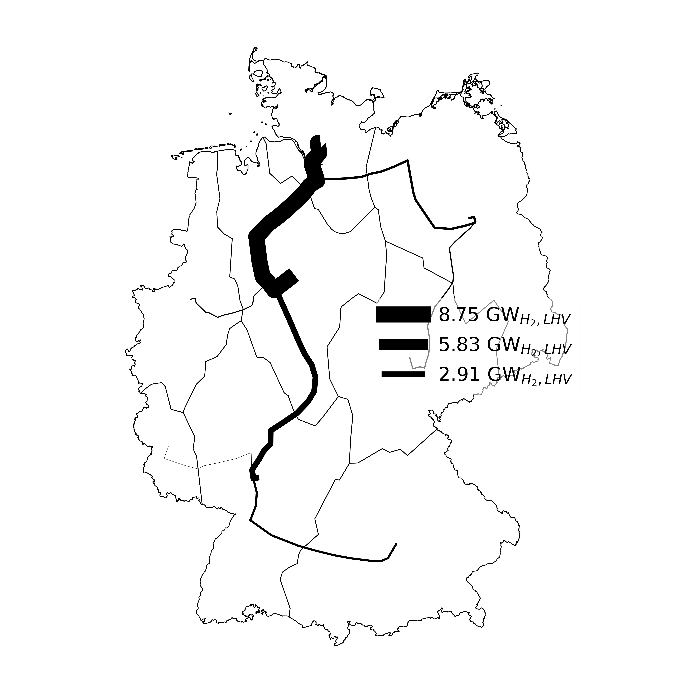
\includegraphics{images/H2Pipeline-95.png}
  \end{minipage}
  \hspace{.1\linewidth}
  \begin{minipage}[b]{.4\linewidth} 
     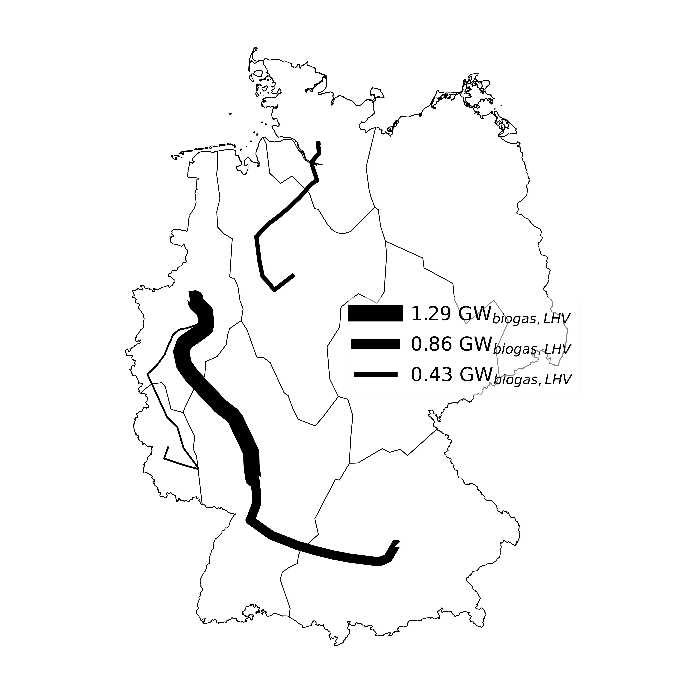
\includegraphics{images/BiogasPipeline-95.png}
  \end{minipage}
  \caption{Verläufe der Wasserstoffpipelines (links) und Biogaspipelines (rechts) der Simulation bei 95 \% CO\textsubscript{2} Reduktion}
  \label{image:Pipelines-95}
\end{figure}

Die Grafiken in der Abbildung \ref{image:Pipelines-95} veranschaulichen die simulierten Verläufe der Wasserstoff- und Biogaspipelines. Die Wasserstoffversorgung verläuft dabei von Nord- nach Südrichtung mit großen Verbrauchern im Bereich Niedersachsens und Nordrhein-Westfalens um das Ruhrgebiet. Die Wasserstoffversorgung beginnt dabei mit ca. 8,75 GW Leistung und nimmt kontinuierlich bis zu den Endverbrauchern in Süddeutschland mit ca. 2,91 GW finaler Leistung ab. Die Versorgung mit Biogas zeigt nach Erstellung der Simulation einen getrennten Verlauf. Hierbei erstellt FINE eine kleine Versorgungstrasse mit ca. 0,43 GW installierter Leistung zwischen Schleswig-Holstein und Niedersachsen und legt die große Energieversorgung beginnend in Nordrhein-Westfalen mit 1,29 GW über Baden-Württemberg mit 0,86 GW und Bayern als Endverbraucher fest. Ein kleiner Versorgungsstrang für das Saarland und Rheinland-Pfalz wird ebenfalls simuliert.

Zum kompletten Verständnis der 95 \% Reduktion wird im Folgenden noch die zukünftige Stromversorgung in Deutschland analysiert, welche in nachfolgender Abbildung \ref{image:Leitungen-95} von FINE simuliert und visualisiert worden ist.

Das Wechselstromnetz wird dabei über alle Regionen in Nord- und Südrichtung verteilt, mit Spitzenleistungen von 18 GW elektrischer Leistung in den Haupttrassen und Verzweigungen zwischen den Knoten mit kleineren Leistungen im Bereich von ca. 12,0 GW bis 6,0 GW. Das Netz zeigt dabei bereits große Ähnlichkeit mit dem heutigen Stromnetz im Jahre 2022 auf. Neu hinzugekommen sind in der Simulation die Trassen der Hochspannungs-Gleichstrom- Übertragung in kurz genannt auch HGÜ. Diese Technik ist relativ neu und beinhaltet insbesondere bei großen und weiten Übertragungen weniger Übertragungs\-verluste als Wechselstromleitungen in gleicher Größe. Implementiert wurden diese Trassen von FINE in Nord- Süd Richtung zwischen Schleswig-Holstein und Baden-Württemberg mit einer maximalen Leistung von 4,0 GW, einer mittleren Leistung im Bereich Sachsens, Thüringen und Bayerns mit 2,66 GW und einer kleinen Versorgung ausgehend von Baden-Württemberg in Richtung Nordrhein-Westfalens mit 1,33 GW.

\begin{figure}[!ht]
  \begin{minipage}[b]{.4\linewidth} 
     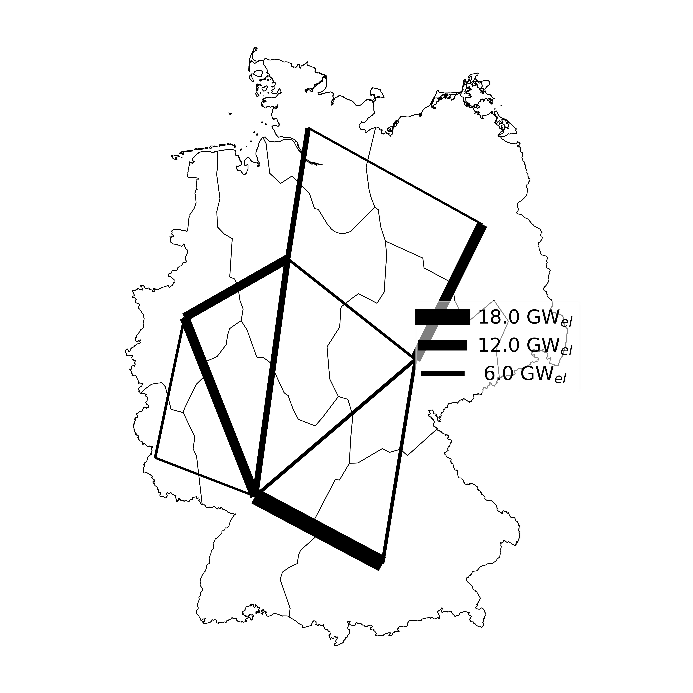
\includegraphics{images/AC-95.png}
  \end{minipage}
  \hspace{.1\linewidth}
  \begin{minipage}[b]{.4\linewidth} 
     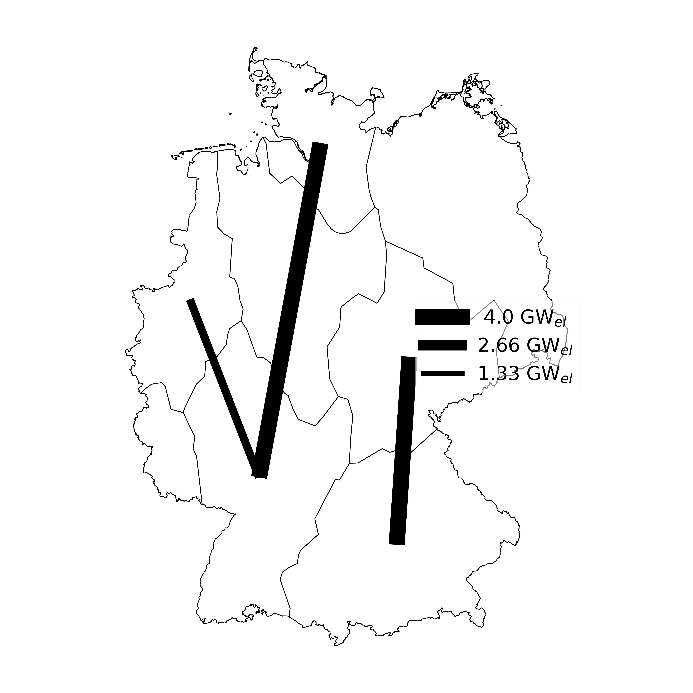
\includegraphics{images/DC-95.png}
  \end{minipage}
  \caption{Verläufe der Wechselstrom- (links) und Gleichstromtrassen (rechts) der Simulation bei 95 \% CO\textsubscript{2} Reduktion}
  \label{image:Leitungen-95}
\end{figure}
\FloatBarrier
\clearpage 


\newpage
\subsection{Reduktionsfall 100 \% (Mehdi Abbadi)}
Im 100 \% Reduktionsfall erreicht das Modell ein CO\textsubscript{2}-neutrales Energiesystem in Deutschland. Dabei existieren keine Gas- und Dampfturbinenkraftwerke mit Methan-Verbrennung, da diese CO\textsubscript{2} ausstoßen würden. In der Konsequenz wird für das gesamte Energiesystem grüner Strom bzw. Wasserstoff erzeugt werden. Zum Einsatz kommen u. a. Biogasanlagen, da diese nur Biogas verbrennen. Daneben sind erneuerbare Energie Anlagen wie Wind On- und Offshore und PV stark ausgebaut und Wasserkraftwerke unterstützen die Energiegewinnung. 

Die gesamte installierte Leistung beträgt in allen Erzeugungsanlagen 370 GW, mit einer Steigerung von ca. 50 GW zum vorherigen Reduktionsfall. Dies kann aufgrund der massiven Produktion aus der erneuerbare Energie resultieren. Da der Anteil an PV einen signifikanten Anstieg von 121 GW auf 188,2 GW berüchtigt und ist in allen Clustern verfügbar ist. Die installierte Leistung an Wind-Offshore steigt auf 81 GW als Spitzenwert und ist in allen Clustern an ihrer Kapazitätsgrenze, was dazu führt, dass Überschüsse in Elektrolyse-Anlagen fließen die in den Clustern vorhanden sind.  Die installierte Leistung Wind onshore beträgt ca. 44,2 GW. Im Vergleich zum 95 \% Fall ist Wind onshore nur im Cluster 6 vorhanden. 

Die Elektrolyse-Leistung steigt somit auf den Maximalwert von 23,3 GW und findet in allen Clustern bis auf 7 Anwendung. Aufgrund der geringen Nachfrage und der vorhandenen Pipeline wird für Cluster 7 keine Elektrolyse angewendet. Um die Nachfrage in voller Höhe bedienen zu können, ist die Energiegewinnung aus PV und Wind nicht ausreichend, weshalb Biogas ebenfalls zur Anwendung kommt. 

Dies führt zudem dazu, dass Langzeitspeicher in Form von Gas-Salzkavernen benötigt werden, um jederzeit die Versorgung sicherzustellen. Für den Bereich Strom stellen Batterie- und Pumpspeicher die wesentlichen Energiespeicher dar. Bei den Batteriespeichern gibt es eine massive Steigerung. Die Speicherkapazität nimmt stark zu auf 129,46 GWh. Der Speicherbedarf lässt sich mit dem Ausbau und der Erzeugung und somit dem Überschuss aus EE-Anlagen plausibilisieren.  

Nach dem der Speicherbedarf bei steigerndem Reduktionsfall zunimmt, erreicht er bei 100 \% CO\textsubscript{2}-Neutralität seinen Maximum. Wesentliche Treiber sind der Einsatz von Wasserstoff und Biogas-Salzkavernenspeicher, da u. a. Biogas nur mit konstanter Menge bezogen werden kann. Hier wird der Vorteil des hohen Speichervolumens genutzt. Die Biogasspeicher ermöglichen eine größere Felxibilität und tragen zum Rückgang der Erdgasnutzung bei. Durch die Speichermöglichkeiten reduziert sich in der Konsequenz die erforderliche Leistung an das H\textsubscript{2}-Pipelinenetz. Einen zusätzlichen Grund liefern die verfügbaren Elektrolyse-Anlagen in den Regionen zur Wasserstofferzeugung.

Die Kostenaufteilung im 100 \% Fall erfolgt ebenfalls nach Erzeugung, Umwandlung, Speicherung und Übertragung. Der größte Anteil an den Gesamtkosten wird durch die Erzeugung mit ca. 86 \% (45 Mrd. €) verursacht. Der Anteil der Speicherkosten belaufen sich auf 9 \% der Gesamtkosten und betragen 4,5 Mrd. €. Die Kosten für Elektrolyse-Anlagen belaufen sich auf ca. 2,93 Mrd. €. Die Umwandlungskosten liegen bei ca. 5,6 \% des TAC. Die restlichen 0,2 \% sind für die Übertragung entstanden. 

Die Gesamtsystemkosten betragen 52 Mrd. €. Diese steigen im Vergleich zu den zuvor erläuterten Reduktionsfällen weiter an. PV verzeichnet einen weiteren Anstieg um ca. 5 Mrd. € auf 13,9 Mrd. €. Die Kosten für Wind offshore verbleiben wie in den letzten zwei Reduktionsfällen mit 22,7 Mrd. €. Dahingegen ist bei Wind onshore ein Anstieg um ca. 1,4 \% auf 5,9 Mrd. € zu entnehmen. Eine Änderung bei den Kosten für Batteriespeicher ist ebenfalls festzustellen. Beliefen sich die Kosten im 95 \% Szenario noch auf 0,07 Mrd. € sind sie im 100 \% Fall bei 2,1 Mrd. €. 

Bei den weggefallenen Kosten handelt es sich um die Importkosten für Erdgas i. H. v. 1,6 Mrd. € und um die Gasanlagen 1,88 Mrd. €. In beiden Komponenten sind für das Energiemodell mit der vorliegenden Restriktion keine Anwendung und somit auch keine Kosten berücksichtigt worden. Dadurch lässt sich zudem die CO\textsubscript{2}-Neutralität erklären.

